\documentclass[12pt,letterpaper]{article}
\usepackage{fullpage}
\usepackage[top=2cm, bottom=4.5cm, left=2.5cm, right=2.5cm]{geometry}
\usepackage{amsmath,amsthm,amsfonts,amssymb,amscd}
\usepackage{lastpage}
\usepackage{enumerate}
\usepackage{fancyhdr}
\usepackage{mathrsfs}
\usepackage{xcolor}
\usepackage{graphicx}
\usepackage{listings}
\usepackage{hyperref}
\usepackage[T1]{fontenc}
\usepackage{textcomp}

\hypersetup{
  colorlinks=true,
  linkcolor=blue,
  linkbordercolor={0 0 1}
}

\definecolor{limitblue}{RGB}{32, 76, 113}
\definecolor{ruddybrown}{rgb}{0.73, 0.4, 0.16}
\colorlet{punct}{red!60!black} 
\definecolor{background}{HTML}{EEEEEE}
\definecolor{delim}{RGB}{20,105,176}
\definecolor{ogreen}{rgb}{0.0, 0.5, 0.0}
\colorlet{numb}{magenta!60!black}
 
\renewcommand\lstlistingname{Code}
\renewcommand\lstlistlistingname{Codes}
\def\lstlistingautorefname{Alg.}

\lstdefinestyle{Python}{
  language        = Python,
  frame           = lines, 
  basicstyle      = \footnotesize,
  keywordstyle    = \color{blue},
  stringstyle     = \color{green},
  commentstyle    = \color{red}\ttfamily
}
\lstdefinestyle{R}{
  language        = R,
  frame           = lines,
  captionpos      = b,
  abovecaptionskip= 10pt, 
  emphstyle       = \textbf,
  framextopmargin = 4pt,
  framexbottommargin = 4pt,
  basicstyle      = \ttfamily\footnotesize,
  keywordstyle    = \color{limitblue},
  stringstyle     = \color{ruddybrown},
  showstringspaces= false,
  commentstyle    = \color{red}\ttfamily,
  tabsize         = 2,
  literate=
    *{0}{{{\color{numb}0}}}{1}
      {1}{{{\color{numb}1}}}{1}
      {2}{{{\color{numb}2}}}{1}
      {3}{{{\color{numb}3}}}{1}
      {4}{{{\color{numb}4}}}{1}
      {5}{{{\color{numb}5}}}{1}
      {6}{{{\color{numb}6}}}{1}
      {7}{{{\color{numb}7}}}{1}
      {8}{{{\color{numb}8}}}{1}
      {9}{{{\color{numb}9}}}{1}
      {:}{{{\color{punct}{:}}}}{1}
      {,}{{{\color{punct}{,}}}}{1}
      {\{}{{{\color{delim}{\{}}}}{1}
      {\}}{{{\color{delim}{\}}}}}{1}
      {[}{{{\color{delim}{[}}}}{1}
      {]}{{{\color{delim}{]}}}}{1}
}

\setlength{\parindent}{0.0in}
\setlength{\parskip}{0.05in}

% Edit these as appropriate
\newcommand\course{Statistics I}
\newcommand\hwnumber{5.3}                  % <-- homework number
\newcommand\NetIDa{Atreya Choudhury}           % <-- NetID of person #1
\newcommand\NetIDb{bmat2005}           % <-- NetID of person #2 (Comment this line out for problem sets)

\pagestyle{fancyplain}
\headheight 35pt
\lhead{\NetIDa}
\lhead{\NetIDa\\\NetIDb}                 % <-- Comment this line out for problem sets (make sure you are person #1)
\chead{\textbf{\Large Assignment \hwnumber}}
\rhead{\course \\ \today}
\lfoot{}
\cfoot{}
\rfoot{\small\thepage}
\headsep 2em

\begin{document}
\textit{1}
\begin{enumerate}[a.]
  \item Draw 1000 random samples of size 2 (X,Y) from Gamma(5,1).
  \item Compute X/(X+Y) of each of these samples and draw a histogram with breaks\\0,0.1,...0.9,1. Record the number of observations in each interval.
\end{enumerate}
\textit{2}
\begin{enumerate}[a.]
  \item Draw 1000 random samples from Beta(5,5) distribution.
  \item Draw a histogram of the outputs from 2a with same breaks as 1b and record the number of observations in each interval.
\end{enumerate}
\textit{3} Compute the difference between the two vectors in 1b and 2b.\\
Submit the plots of the 2 histograms, the vector of differences and the code.\\
Why do you expect the two histograms to be close?\\

\vspace{2em}
Let X and Y be independent gamma(5,1) distributions.

Let,
\begin{align*}
  U &= \frac{X}{X+Y}\\
  V &= X+Y
\end{align*}

Then, 
$$\begin{pmatrix}
  X\\
  Y
\end{pmatrix}
=
\begin{pmatrix}
  UV\\
  V-UV
\end{pmatrix}$$

and the jacobian is given,

\begin{align*}
  J &= \begin{pmatrix}
    v & u\\
    -v & 1-u
  \end{pmatrix}\\
  \implies |J| &= v
\end{align*}
\begin{align*}
  \therefore f_{U,V}(u, v) &= |J| f_{X,Y}(uv, v-uv)\\
  &= v f_X(uv) f_Y(v-uv)\\
  &= v \frac{(uv)^4 e^{-uv}}{\Gamma(5)}1_{uv \geq 0}\frac{(v-uv)^4 e^{-(v-uv)}}{\Gamma(5)}1_{v-uv \geq 0}
\end{align*}
\newpage
Now,
$$1_{uv \geq 0} = 1_{v \geq 0} 1_{u \geq 0}$$
as neither $u$ nor $v$ can be negative(as X, Y $\geq$ 0)


Also,
\begin{align*}
  1_{v-uv \geq 0} &= 1_{1-u \geq 0}\hspace{3em}[\because v \geq 0]\\
  &= 1_{u \leq 1}
\end{align*}

$$\therefore f_{U,V}(u, v) = \frac{v^9 e^{-v}}{\Gamma(10)}1_{v \geq 0}\frac{\Gamma(10)}{\Gamma(5)^2}u^4(1-u)^4 1_{0 \leq u \leq 1}$$

\begin{align*}
  \therefore f_U(u) &= \int_{-\infty}^{\infty} f_{U,V}(u, v) dv\\
  &= \int_{-\infty}^{\infty}\frac{v^9 e^{-v}}{\Gamma(10)}1_{v \geq 0}\frac{\Gamma(10)}{\Gamma(5)^2}u^4(1-u)^4 1_{0 \leq u \leq 1}dv\\
  &= \frac{u^4(1-u)^4}{B(5,5)}1_{0 \leq u \leq 1}\int_{0}^{\infty}\frac{v^9 e^{-v}}{\Gamma(10)}dv\\
  &= \frac{u^4(1-u)^4}{B(5,5)}1_{0 \leq u \leq 1}
\end{align*}

$\therefore \frac{X}{X+y} \sim Beta(5,5)$

The distributions in R are generated from the same distribution. Hence, the histograms are similar.
\newpage
\begin{figure*}[h]
  \centering
  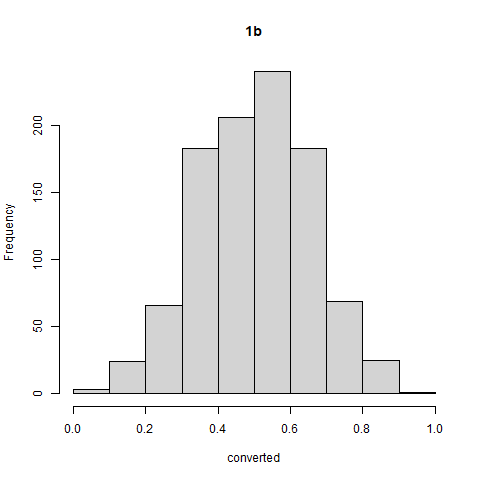
\includegraphics[width=15cm]{Histogram_1.png}
  \caption{Histogram of 1b}
\end{figure*}

Number of observations in each interval:\\
3 24 66 183 206 240 183 69 25 1
\newpage
\begin{figure*}[h]
  \centering
  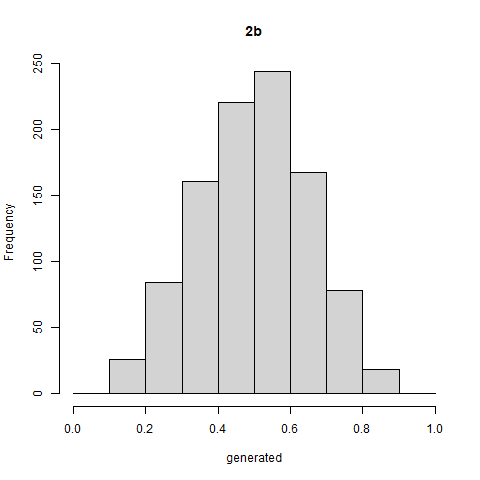
\includegraphics[width=15cm]{Histogram_2.png}
  \caption{Histogram of 2b}
\end{figure*}

Number of observations in each interval:\\
0 26 84 161 221 244 168 78 18 0
\newpage

Difference in number of observations in each interval:\\
3 -2 -18 22 -15 -4 15 -9 7 1\\
\vspace{4em}
\lstinputlisting[language=R, style=R, title=R Code for Histograms]{code.R}
\end{document}